% L22eqv.tex
% $Author$ $Date$

\section{Geometry of state space with $L=22$}
\label{sec:L22}

%%%%%%%%%%%%%%%%%%%%%%%%%%%%%%%%%%%%%%%%%%%%%%%%%%%%%%%%%%%%%%
\begin{figure}[t]
\begin{center}
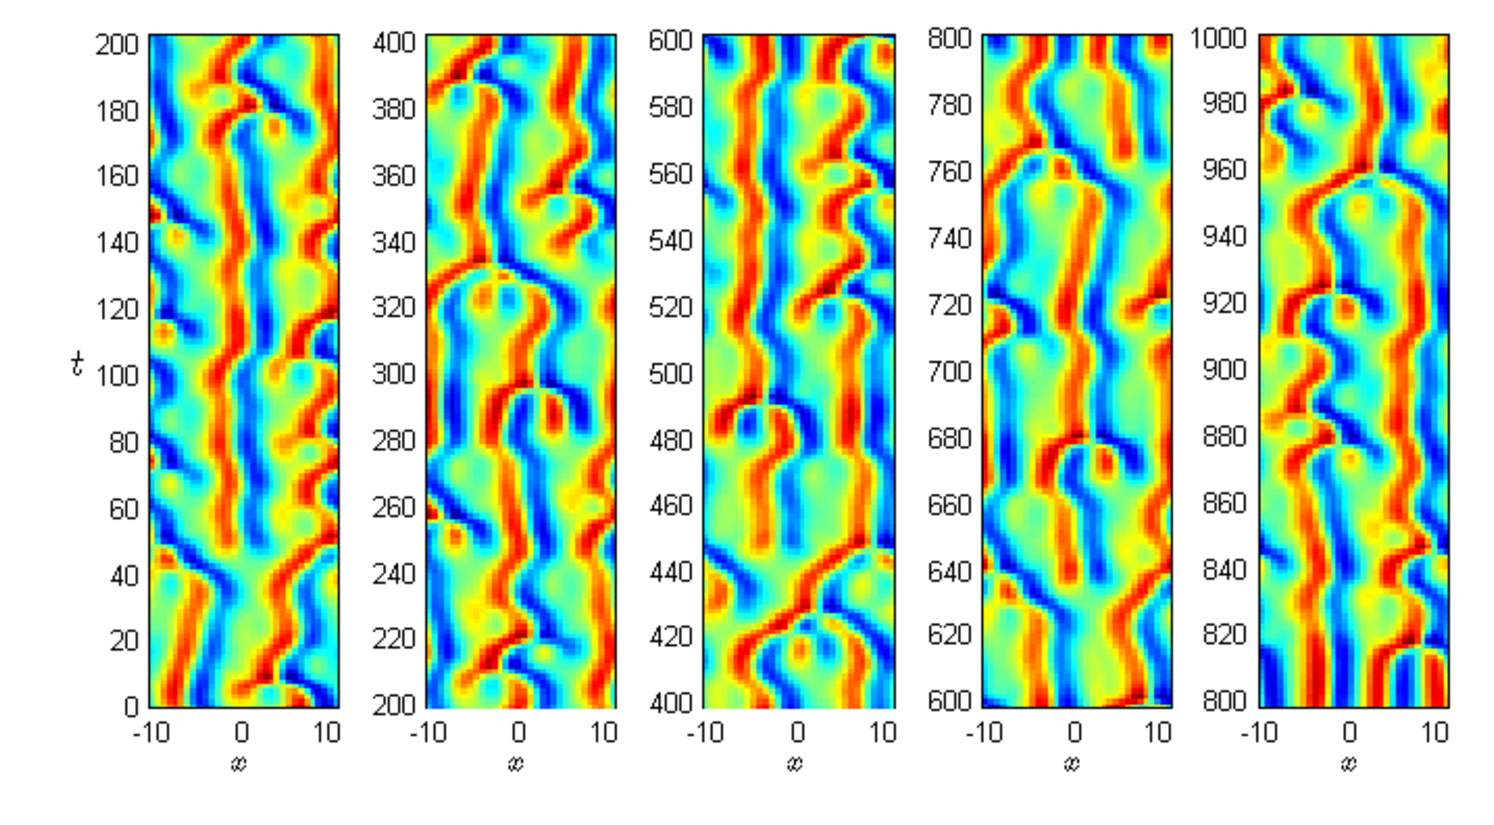
\includegraphics[width=0.9\textwidth, clip=true]{figs_bmp/ks_L22_long_orbit.eps}
\end{center}
\caption{
A typical chaotic orbit of the KS flow, system size $L=22$.
     } \label{f:ks_L22}
\end{figure}
%%%%%%%%%%%%%%%%%%%%%%%%%%%%%%%%%%%%%%%%%%%%%%%%%%%%%%%%%%%%%%%%%%
We now turn to exploring Hopf's vision
numerically, on a specific KS system.
An instructive example is offered by the dynamics for
the  $L=22$  system
that we specialize to for the rest of this paper.
The size of this
small system is $\sim 2.5$ mean wavelengths
($\tildeL/\sqrt{2}= 2.4758\ldots$),
and the competition between states with wavenumbers 2 and 3
leads to
what, in the context of boundary shear flows, would be
called\rf{HaKiWa95} the `empirically observed sustained
turbulence,' but in the present context may equally well be
characterized as a `chaotic attractor.' A typical long orbit
is shown in \reffig{f:ks_L22}.
Asymptotic attractor structure of small systems like
the one studied here
is very sensitive to system parameter variations, and,
as is true of
any realistic unsteady flow, there is no rigorous way of
establishing that this `turbulence' is sustained for all time,
rather than being
merely a very long transient on a way to an
attracting periodic state.
For large system size, as the one shown in \reffig{f:ks_largeL}, it is
hard to imagine a scenario under which attracting periodic states
(as shown in \refref{FSTks86}, they do exist) would have significantly
large immediate basins of attraction.
Regardless of the
(non)existence of a $t \to \infty$ chaotic attractor, study
of the invariant unstable solutions and the associated Smale
horseshoe structures in system's \statesp\ offers valuable
insights into the observed unstable `coherent structures.'

Because of the strong $k^4$ contraction, for a small system
size the long-time dynamics
is confined to low-dimensional
inertial manifold\rf{jolly_evaluating_2000}.
Indeed, numerically the covariant Lyapunov vectors\rf{ginelli-2007-99} of the
$L=22$ chaotic attractor separate into 8 ``physical''
vectors with small Lyapunov exponents
$(\Lyap_j) = (0.048,$ 0, 0, $-0.003$, $-0.189$, $-0.256$,
$-0.290$, $-0.310$),
and the remaining 54 ``hyperbolically isolated'' vectors
with rapidly decreasing exponents
$(\Lyap_j) = (-1.963$,   $-1.967$,   $-5.605$,   $-5.605$,  $-11.923$,  $-11.923$,
 $\cdots) \approx -(j/\tildeL)^4$,
in full agreement with the Yang \etal\rf{YaTaGiChRa08}
investigations of KS for large systems sizes.
%, up to $L=192$.
The chaotic dynamics mostly takes place close to a
8-dimensional manifold, with strong contraction in other
dimensions.  The two zero exponents are due to the time and
space translational symmetries of the \KSe\ and the 2 corresponding
dimensions can be quotiented out by means of discrete-time
Poincar\'e sections and $O(2)$ group orbit slices.
It was shown
in \refrefs{Christiansen97,lanCvit07} that within unstable-manifold
curvilinear coordinate frames, the dynamics on the attractor
can sometimes be well approximated by local 1- or 2-dimensional
Poincar\'e return maps.
Hence a relatively small number of real Fourier modes, such as 62
to 126 used in calculations presented here, suffices
to obtain  invariant
solutions numerically accurate to within $10^{-5}$.

We next investigate the properties of \eqva\ and \reqva\ and
determine numerically a large set of the short periods \rpo s
for KS in a periodic cell of size $L=22$.

\section{\Eqva\ and \reqva\ for $L=22$}

In addition to the trivial \eqv\ $u=0$ (denoted \EQV{0}),
we find three \eqva\ with dominant wavenumber $k$
(denoted \EQV{k}) for $k = 1, 2, 3$.  All {\eqva}, shown in
\reffig{f:KS22Equil}, are symmetric with respect to the reflection
symmetry \refeq{KSparity}.
In addition, \EQV{2} and \EQV{3} are symmetric with respect
to translation \refeq{KSshift}, by $L/2$ and $L/3$, respectively.
\EQV{2} and \EQV{3} essentially lie in
the 2$^\mathrm{nd}$ and 3$^\mathrm{rd}$ Fourier component complex planes,
with small  deformations of the $k=2j$ and $k=3j$ harmonics, respectively.

%%%%%%%%%%%%%%%%%%%%%%%%%%%%%%%%%%%%%%%%%%%%%%%%%%%%%%%%%%%%%%%%%%
\begin{figure}[t]
\begin{center}
  (\textit{a})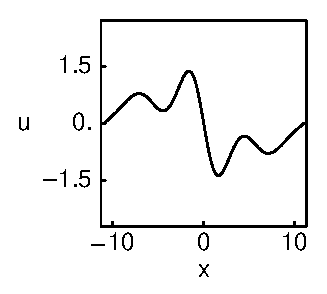
\includegraphics[width=0.35\textwidth, clip=true]{figs_bmp/1wKS22equil.eps}
~~~~(\textit{b})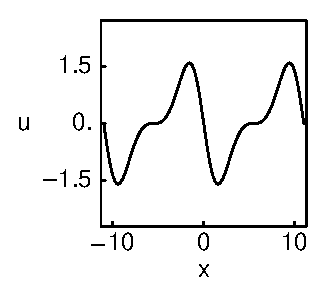
\includegraphics[width=0.35\textwidth, clip=true]{figs_bmp/2wKS22equil.eps}
\\
  (\textit{c})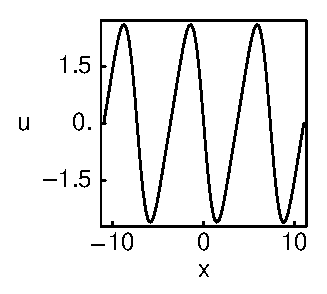
\includegraphics[width=0.35\textwidth, clip=true]{figs_bmp/3wKS22equil.eps}
~~~~(\textit{d})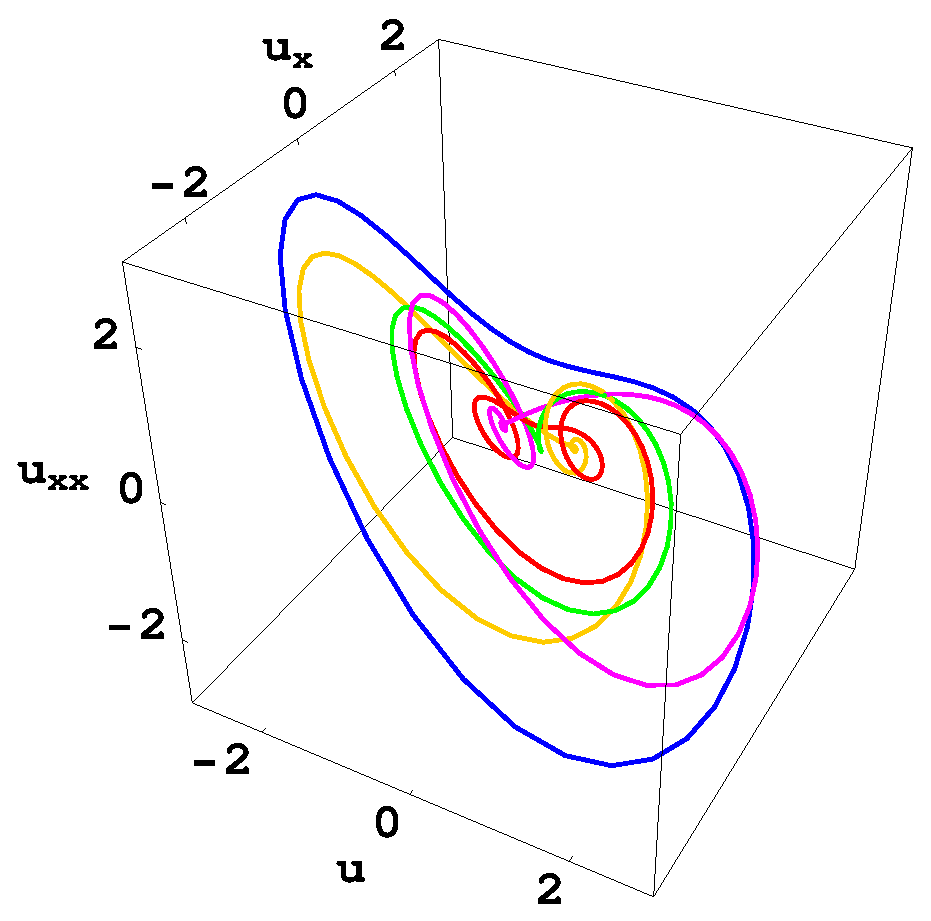
\includegraphics[width=0.35\textwidth, clip=true]{figs_bmp/equilSpatial.eps}
\end{center}
\caption{
(a) \EQV{1}, (b) \EQV{2}, and (c)
\EQV{3} \eqva. The \EQV{0} \eqv\ is the $u(x)=0$ solution.
(d) $(u,u_x,u_{xx})$ representation
of (red) \EQV{1}, (green) \EQV{2},  (blue) \EQV{3} \eqva,
(purple) \REQV{+}{1},  and (orange) \REQV{-}{1} \reqva.
$L=22$ system size.
    }
\label{f:KS22Equil}
\end{figure}
%%%%%%%%%%%%%%%%%%%%%%%%%%%%%%%%%%%%%%%%%%%%%%%%%%%%%%%%%%%%%%%%

The stability of the {\eqva} is characterized by the eigenvalues
$\eigExp[j]$ of the \stabmat.  The leading 10 eigenvalues for each
\eqv\ are listed in \reftab{tab:Eksym};
those with $\eigRe > -2.5$ are also plotted in
\reffig{f:KS22EkEigs}.
We have computed (available upon request) the corresponding
eigenvectors as well. As an \eqv\ with $\mathrm{Re}\,
\Lyap_j > 0$ is unstable in the direction of the
corresponding eigenvector $\jEigvec{j}$, the eigenvectors
provide flow-intrinsic (PDE discretization independent)
coordinates which we use for visualization of unstable
manifolds and homo/heteroclinic connections between \eqva.
We find such coordinate frames, introduced by
Gibson \etal\rf{GHCW07,GibsonMovies}, better suited to visualization
of nontrivial solutions than the more standard Fourier mode
(eigenvectors of the $u(x,t)=0$ solution) projections.


The eigenvalues of \EQV{0} are determined by the linear part of the KS
equation \refeq{expanMvar}: $\Lyap_k=(k/\tilde{L})^2-(k/\tilde{L})^4$.
For $L=22$, there are three pairs of unstable eigenvalues, corresponding,
in decreasing order, to three unstable modes $k=2,3$, and 1.  For each
mode, the corresponding eigenvectors lie in the plane spanned by
$\Re \, a_k$ and $\Im \, a_k$. \refTab{tab:Eksym}
lists the symmetries of the stability eigenvectors of
\eqva\ \EQV{1} to \EQV{3}.

\begin{figure}[t]
\begin{center}
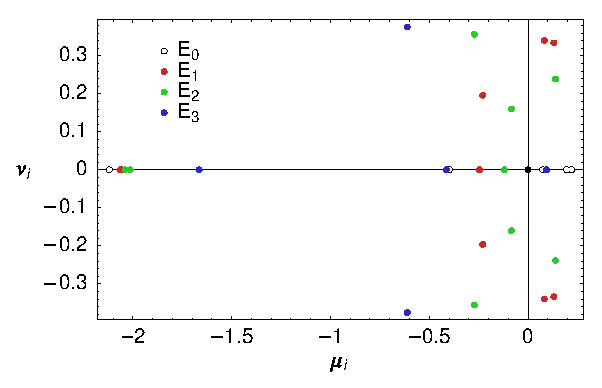
\includegraphics[width=4in]{figs_bmp/L22-eqvaEigenvalues.eps}
\end{center}
\caption{
Leading  \eqv\ stability eigenvalues,
$L=22$ system size.
}
\label{f:KS22EkEigs}
\end{figure}

\begin{table}[t]
\caption{
Leading eigenvalues
$\eigExp[j]= \eigRe[j] \pm i\eigIm[j]$
and symmetries of the corresponding eigenvectors
of KS {\eqva} and \reqva\ for $L = 22$ system size.
We have used as our reference states the ones that lie within
the antisymmetric subspace  $\bbU^+$,
and also listed the symmetries of
the $L/4$ translated ones.
        }\label{tab:Eksym}
\begin{center} \footnotesize
\begin{tabular}{ccccc}
\EQV{1}& $\eigRe[j]$ & $\eigIm[j]$ & Symmetry & $\Shift_{1/4}\EQV{n}$ Symmetry\\\hline
  $\eigExp[1,2]$ & $\ \ 0.1308$& $0.3341$ & -  & -\\
  $\eigExp[3,4]$ & $\ \ 0.0824$& $0.3402$ & $\bbU^+$  & $\bbU^{(1)}$\\
  $\eigExp[5]$   & $0$     &          & -  & -\\
  $\eigExp[6,7]$ &$-0.2287$& $0.1963$ & $\bbU^+$  & $\bbU^{(1)}$\\
  $\eigExp[8]$   &$-0.2455$&          & -  & -\\
  $\eigExp[9]$   &$-2.0554$&          & $\bbU^+$  & $\bbU^{(1)}$\\
  $\eigExp[10]$  &$-2.0619$&          & -  & -\\[2ex]
\EQV{2}&  &  & \\\hline
  $\eigExp[1,2]$ & $\ \ 0.1390$& $0.2384$ & $\bbU^+$         & $\bbU^{(1)}$\\
  $\eigExp[3]$   & $0$      &          & $\Shift_{1/2}$        & $\Shift_{1/2}$\\
  $\eigExp[4,5]$ &$-0.0840$ & $0.1602$ & $\bbU^{(1)}$           & $\bbU^+$\\
  $\eigExp[6]$   &$-0.1194$ &          & $\Shift_{1/2}$        & $\Shift_{1/2}$\\
  $\eigExp[7,8]$ &$-0.2711$ & $0.3563$ & $\bbU^+,\,\bbU^{(1)},\,\Shift_{1/2}$  & $\bbU^+,\,\bbU^{(1)},\,\Shift_{1/2}$\\
  $\eigExp[9]$   &$-2.0130$ &          & $\bbU^{(1)}$           & $\bbU^+$\\
  $\eigExp[10]$  &$-2.0378$ &          & $\bbU^+$         & $\bbU^{(1)}$\\[2ex]
\EQV{3}&  &  & \\\hline
  $\eigExp[1]$   &$\ \ 0.0933$&          & $\bbU^+$     & $\bbU^{(1)}$\\
  $\eigExp[2]$   &$\ \ 0.0933$&          & -         & -  \\
  $\eigExp[3]$   &$0$       &          & $\Shift_{1/3}$    & $\Shift_{1/3}$\\
  $\eigExp[4]$   &$-0.4128$ &          & $\bbU^+,\,\Shift_{1/3}$  & $\bbU^{(1)},\,\Shift_{1/3}$\\
  $\eigExp[5,6]$ &$-0.6108$ & $0.3759$ & $\bbU^+$     & $\bbU^{(1)}$\\
  $\eigExp[7,8]$ &$-0.6108$ & $0.3759$ & -         & -\\
  $\eigExp[9]$   &$-1.6641$ &          & -         & -\\
  $\eigExp[10]$  &$-1.6641$ &          & $\bbU^+$     & $\bbU^{(1)}$ \\[2ex]
$\REQV{\pm}{1}$&  &  & \\\hline
  $\eigExp[1,2]$ & $\ \ 0.1156$ & $0.8173$ & -  & -\\
  $\eigExp[3,4]$ & $\ \ 0.0337$ & $0.4189$ & -  & -\\
  $\eigExp[5]$   & $0$      &          & -  & -\\
  $\eigExp[6]$   &$-0.2457$ &          & -  & -\\
  $\eigExp[7,8]$ &$-0.3213$ & $0.9813$ & -  & -\\[2ex]
$\REQV{\pm}{2}$&  &  & \\\hline
  $\eigExp[1]  $ & $\ \ 0.3370$ &          & -  & -\\
  $\eigExp[2]  $ & $0$      &          & -  & -\\
  $\eigExp[3,4]$ &$-0.0096$ & $0.6288$ & -  & -\\
  $\eigExp[5,6]$ &$-0.2619$ & $0.5591$ & -  & -\\
  $\eigExp[7,8]$ &$-0.3067$ & $0.0725$ & -  & -\\
\end{tabular}
\end{center}
\end{table}


%%%%%%%%%%%%%%%%%%%%%%%%%%%%%%%%%%%%%%%%%%%%%%%%%%%%%%%%%%%%%%%%%%
\begin{figure}[t]
\begin{center}
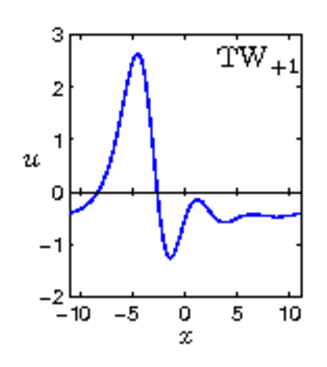
\includegraphics[width=0.3\textwidth, clip=true]{figs_bmp/ks22_TW1_profile.eps}
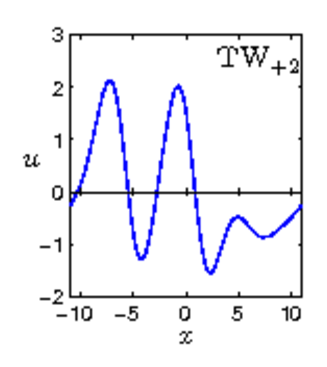
\includegraphics[width=0.3\textwidth, clip=true]{figs_bmp/ks22_TW2_profile.eps}\\
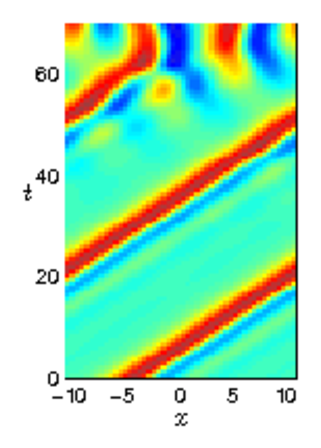
\includegraphics[width=0.3\textwidth, clip=true]{figs_bmp/ks22_TW1_orbit_c.eps}
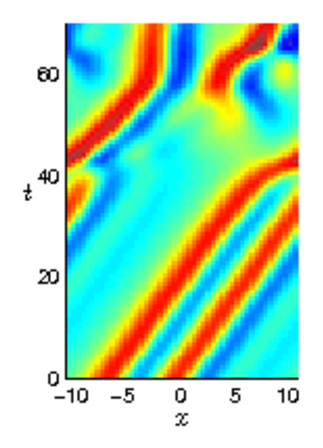
\includegraphics[width=0.3\textwidth, clip=true]{figs_bmp/ks22_TW2_orbit_c.eps}
\end{center}
\caption{
\Reqva : \REQV{+}{1} with velocity $\velRel = 0.737$ and \REQV{+}{2} with
velocity $\velRel = 0.350$.
The upper panels show the \reqva\ profiles.  The lower panels show
evolution of slightly perturbed \reqva\ and their decay into generic
turbulence. Each \reqv\ has a reflection symmetric partner related by
$u(x) \to -u(-x)$ travelling with velocity $-\velRel$.
} \label{f:ks22TW}
\end{figure}
%%%%%%%%%%%%%%%%%%%%%%%%%%%%%%%%%%%%%%%%%%%%%%%%%%%%%%%%%%%%%%%%%%

Consistent with the bifurcation diagram of \reffig{fig:ksBifDiag},
we find two pairs of \reqva\ \refeq{reqva} with velocities
$\velRel =\pm 0.73699$ and $\pm 0.34954$
which we label \REQV{\pm}{1} and \REQV{\pm}{2},
for `traveling waves.'
The profiles of the two \reqva\ and their time evolution
with eventual decay into the chaotic attractor are
shown in \reffig{f:ks22TW}.  The leading eigenvalues of
\REQV{\pm}{1} and \REQV{\pm}{2} are listed in \reftab{tab:Eksym}.

\refTab{tab:L22cminus} lists \eqv\ energy $E$,
the local Poincar\'e section return time $T$,
radially expanding Floquet multiplier $\ExpaEig_e$, and
the least contracting Floquet multiplier $\ExpaEig_c$
for all $L=22$ \eqva\ and \reqva.
The return time $T=2\pi/\eigIm[e]$ is given by the imaginary
part of the leading complex eigenvalue,
the expansion
multiplier per one turn of the most unstable spiral-out by
$\ExpaEig_e\approx\exp(\eigRe[e] T)$, and the contraction
rate along the slowest contracting stable eigendirection by
$\ExpaEig_c\approx\exp(\eigRe[c]T)$.
For \EQV{3} and \REQV{\pm}{2}, whose leading eigenvalues are
real, we use $T=1/\Lyap_1$ as the characteristic time scale.
While the complex eigenvalues set time scales of recurrences,
this time scale is useful for comparison of leading expanding
and the slowest contracting multiplier.
We learn that the shortest
`turn-over' time is $\approx 10-20$, and that if there exist
horseshoe sets of unstable \po s associated with
these \eqva,  they have unstable
multipliers of order of $\ExpaEig_e \sim 5-10$, and that
they are surprisingly thin in the folding direction, with
contracting multipliers of order of $10^{-2}$,
as also observed in \refref{lanCvit07}.

\begin{table}[ht]
    \caption{
    Properties of \eqva\ and \reqva\ determining
    the system dynamics in their vicinity.  $T$ is characteristic
    time scale of the dynamics, $\ExpaEig_e$ and $\ExpaEig_c$ are the
    leading expansion and contraction multipliers, and $E$ is the
    energy \refeq{ksEnergy}.
            }
\begin{center} \footnotesize
    \begin{tabular}{l|rrrr}
                 & $E$~~   & $T$~~  & $\ExpaEig_e$  & $\ExpaEig_c$  \\ \hline
 $\EQV{1}\ $     &\ 0.2609 &\ 18.81 &\ 11.70    &\ 0.01 \\ %Young ES had: \ExpaEig_e=4.79, \ExpaEig_c=0.04
 $\EQV{2}\ $     &\ 0.4382 &\ 26.35 &\ 39.00    &\ 0.11 \\ %Young ES had: \ExpaEig_e=5.99, \ExpaEig_c=0.03
 $\EQV{3}\ $     &\ 1.5876 &\ 10.72 &\ 2.72     &\ 0.01 \\ %ES had \ExpaEig_e=9.92
 $\REQV{\pm}{1}$ &\ 0.4649 &\  7.69 &\ 2.43     &\ 0.15 \\
 $\REQV{\pm}{2}$ &\ 0.6048 &\  2.97 &\ 2.72     &\ 0.97 \\ %PC entered 2.72 = e^1
    \end{tabular}
\end{center}
\label{tab:L22cminus}
\end{table}

\subsection{Unstable manifolds of \eqva\ and their heteroclinic
            connections}
\label{sec:unstMnflds}

As shown in \refTab{tab:Eksym},
the \EQV{1} \eqv\ has two unstable
planes within which the solutions are spiralling out (\ie, two
pairs of complex conjugate eigenvalues).  The \EQV{2} has one such plane,
while the \EQV{3} has two real positive eigenvalues, so the solutions are
moving radially away from the \eqv\ within the plane spanned
by the corresponding eigenvectors.  Since \EQV{1} has
a larger unstable subspace, it is expected to have much less influence on the
long time dynamics compared to \EQV{2} and \EQV{3}.

\begin{figure}[t]
\begin{center}
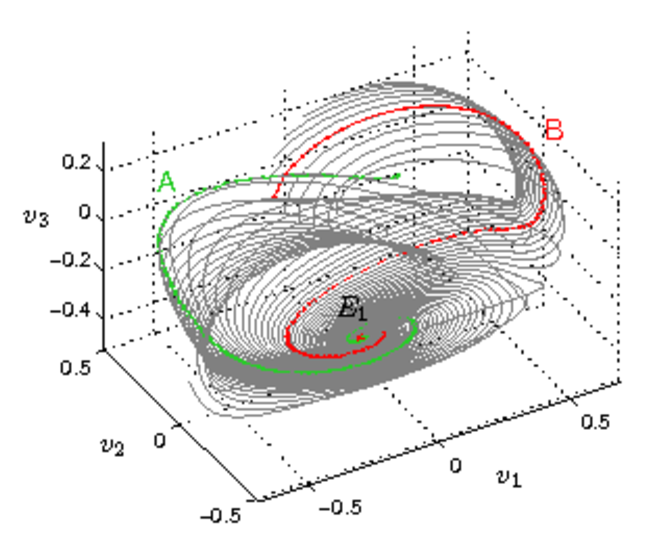
\includegraphics[width=0.5\textwidth, clip=true]{figs_bmp/ks22_E1_plane1_manifold_c.eps}
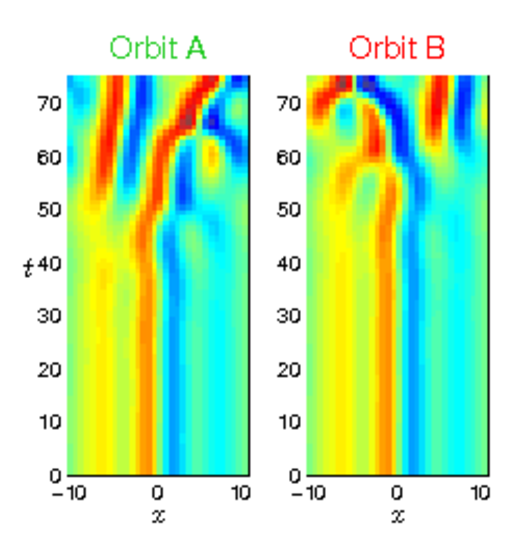
\includegraphics[width=0.4\textwidth, clip=true]{figs_bmp/ks22_E1_plane1_orbits_c.eps}
\end{center}
\caption{
The left panel shows the unstable
manifold of \eqv\ \EQV{1} starting within the plane
corresponding to the first pair of unstable eigenvalues. The
coordinate axes $v_1$, $v_2$, and $v_3$ are
projections onto three orthonormal vectors
$\mathbf{v}_1$, $\mathbf{v}_2$, and $\mathbf{v}_3$,
respectively,
constructed from vectors
$\Re \,\jEigvec{1}$, $\Im \,\jEigvec{1}$,
and $\Re \,\jEigvec{6}$
by Gram-Schmidt orthogonalization.
The right panel shows spatial representation of two orbits $A$ and $B$.
The change of color from blue to red indicates increasing values of
$u(x)$, as in the colorbar of \reffig{f:ks_largeL}.
}
\label{f:KS22E1man1}
\end{figure}

Many methods have been developed for visualization of stable
and unstable manifolds, see \refref{krauskopf_survey_2005}
for a survey. For high-dimensional contracting flows
visualization of stable manifolds is impossible, unless the
system can be restricted to an approximate  low-dimensional
inertial manifold, as, for example, in \refref{kev01ks}. The unstable
manifold visualization also becomes harder as its dimension
increases. Here we concentrate on visualizations of $1$-- and
$2$--dimensional unstable manifolds. Our visualization is
unsophisticated compared to the methods of
\refref{krauskopf_survey_2005}, yet sufficient for our
purposes since, as we shall see, the unstable manifolds we
study terminate in another equilibrium and thus there is no
need to track them for long times.


To construct an invariant manifold containing solutions
corresponding to the pair of unstable complex conjugate eigenvalues,
$\eigExp = \eigRe \pm i\eigIm$,
$\eigRe > 0$, we start with a set of
initial conditions near \eqv\ \EQV{k},
\beq
  a(0) = a_{{\EQV{k}}} + \epsilon\,\exp(\delta)\jEigvec{j}
\,,
\ee{linUnstMan}
where $\delta$ takes a set of values uniformly distributed in the
interval $[0,2\pi\eigRe/\eigIm]$, $\jEigvec{j}$ is a unit vector in the
unstable plane, and $\epsilon > 0$ is small.

\begin{figure}[t]
\begin{center}
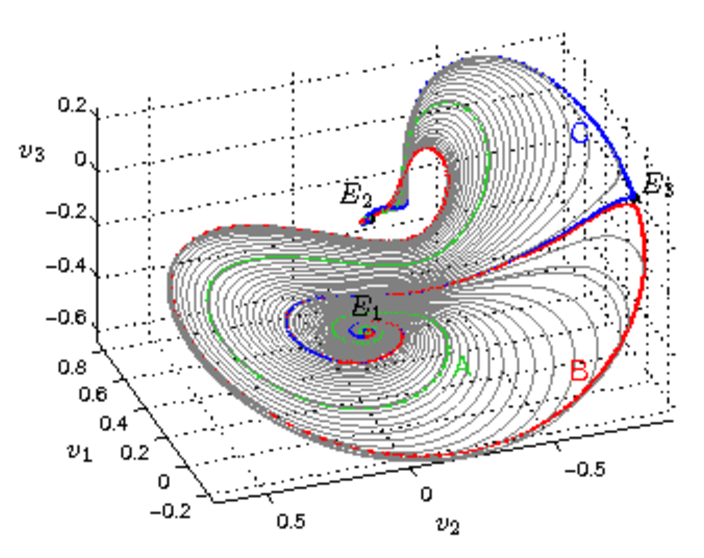
\includegraphics[width=0.48\textwidth, clip=true]{figs_bmp/ks22_E1_plane2_manifold_c.eps}
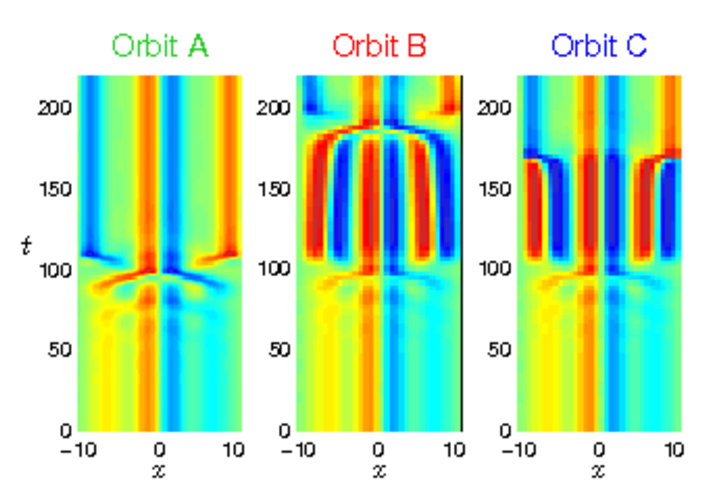
\includegraphics[width=0.48\textwidth, clip=true]{figs_bmp/ks22_E1_plane2_orbits_c.eps}
\end{center}
\caption{
The left panel shows the unstable
manifold of \eqv\ \EQV{1} starting within the plane
corresponding to the second pair of unstable eigenvalues. The
coordinate axes $v_1$, $v_2$, and $v_3$ are
projections onto three orthonormal vectors
$\mathbf{v}_1$, $\mathbf{v}_2$, and $\mathbf{v}_3$,
respectively, constructed from vectors
\Re\, $\jEigvec{3}$, \Im\, $\jEigvec{3}$, and \Re\, $\jEigvec{6}$
by Gram-Schmidt orthogonalization.
The right panel shows spatial representation of three orbits. Orbits
$B$ and $C$ pass close to the \eqv\ \EQV{3}.
   }
\label{f:KS22E1man2}
\end{figure}

The manifold starting within the first unstable plane of \EQV{1}, with
eigenvalues $0.1308\pm i\,0.3341$, is shown in
\reffig{f:KS22E1man1}. It appears to fall directly into the
chaotic attractor.  The behavior of the manifold starting within
the second unstable plane of \EQV{1}, eigenvalues $0.0824\pm i \, 0.3402$, is
remarkably different: as can be seen in \reffig{f:KS22E1man2},
almost all orbits within the manifold converge to the \eqv\ \EQV{2}.  The
manifold also contains a heteroclinic connection from \EQV{1} to \EQV{3},
and is bordered by the $\eigExp[1]$-eigendirection
unstable manifold of \EQV{3}.

\begin{figure}[ht]
\begin{center}
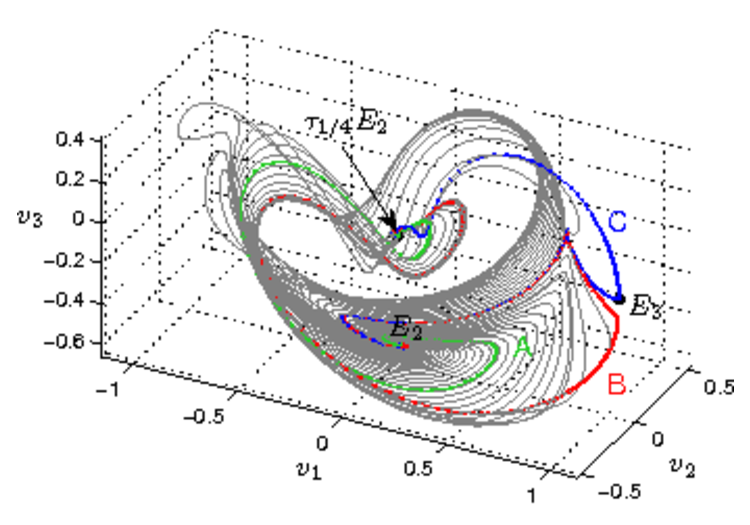
\includegraphics[width=0.48\textwidth, clip=true]{figs_bmp/ks22_E2_manifold_c.eps}
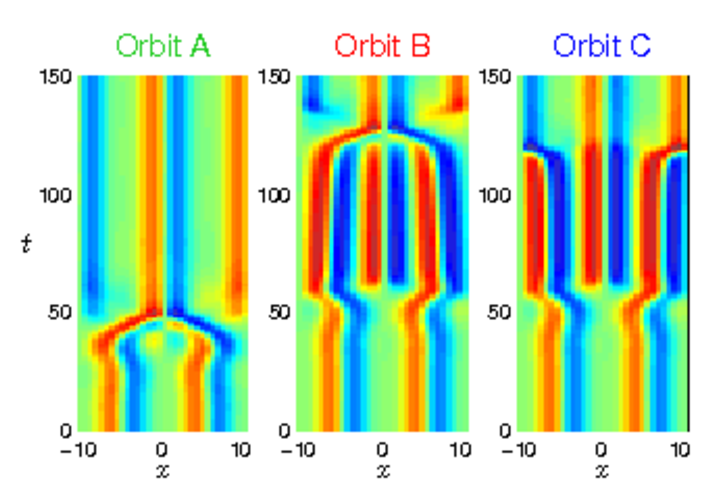
\includegraphics[width=0.48\textwidth, clip=true]{figs_bmp/ks22_E2_orbits_c.eps}
\end{center}
\caption{
The left panel shows the two-dimensional
unstable manifold of \eqv\ \EQV{2}. The coordinate axes
$v_1$, $v_2$, and $v_3$ are
projections onto three orthonormal vectors
$\mathbf{v}_1$, $\mathbf{v}_2$, and $\mathbf{v}_3$,
respectively, constructed from vectors
\Re\, $\jEigvec{1}$, \Im\, $\jEigvec{1}$, and \Re\, $\jEigvec{7}$
by Gram-Schmidt orthogonalization.
The right panel shows spatial representation of three orbits. Orbits
$B$ and $C$ pass close to the \eqv\ \EQV{3}. See
\reffig{f:KS22Manifold} for a different visualization.
       }
\label{f:KS22E2man}
\end{figure}


%%%%%%%%%%%%%%%%%%%%%%%%%%%%%%%%%%%%%%%%%%%%%%%%%%%%%%%%%%%%%%%%
\begin{figure}[t]
\begin{center}
%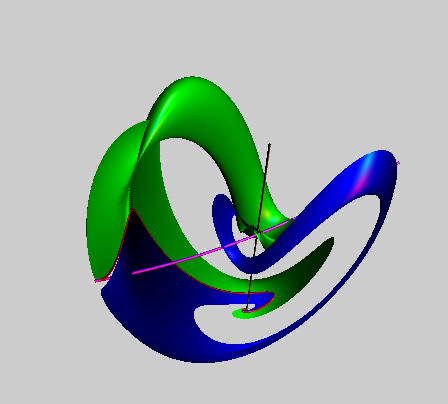
\includegraphics[width=0.6\textwidth, clip=true]{figs_bmp/ks22manifold.ps}
(\textit{a}) 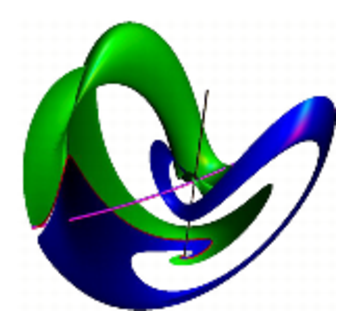
\includegraphics[width=0.4\textwidth, clip=true]{figs_bmp/ks22manifold1.eps}
(\textit{b}) 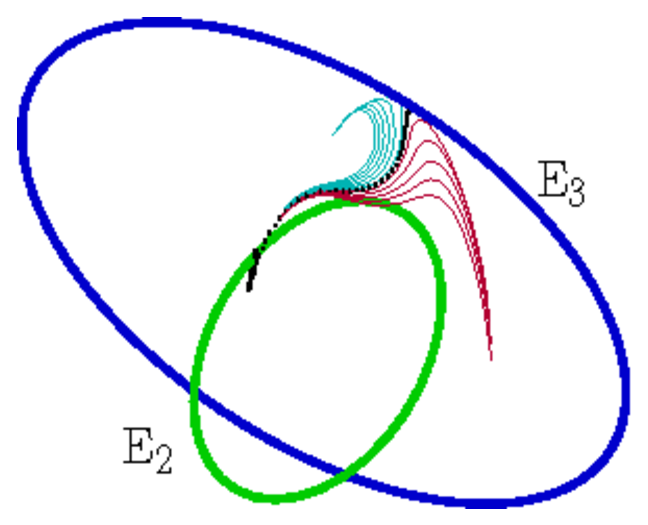
\includegraphics[width=0.4\textwidth, clip=true]{figs_bmp/ks22E2-E3hetero.eps}
\end{center}
\caption{
(a) (blue/green) The unstable manifold of \EQV{2}~\eqv, projection
	in the coordinate axes of \reffig{f:KS22E2man}.
    (black line) The circle of \EQV{2}~\eqva\
related by the translation invariance.
(purple line) The circle  of \EQV{3}~\eqva.
(red) The heteroclinic connection
from the \EQV{2}~\eqv\ to the \EQV{3}~\eqv\ splits
the manifold into two parts,
colored (blue) and (green).
(b) \EQV{2}~\eqv\ to \EQV{3}~\eqv\ heteroclinic
connection, $(\Re\, \jEigvec{2}, \Re\, \jEigvec{3}, ( \Im\, \jEigvec{2} + \Im\, \jEigvec{3})/\sqrt{2})$ projection. 
Here we omit the unstable manifold of \EQV{2},
keeping only a few neighboring trajectories in order to indicate
the unstable manifold of \EQV{3}. The \EQV{2} and \EQV{3}
families of \eqva\ arising from the continuous translational
symmetry of KS on a periodic domain are indicated by the two circles.
        }
\label{f:KS22Manifold}
\end{figure}
%%%%%%%%%%%%%%%%%%%%%%%%%%%%%%%%%%%%%%%%%%%%%%%%%%%%%%%%%%%%%%%%%%

The two-dimensional unstable manifold of \EQV{2} is shown in
\reffig{f:KS22E2man}.  All orbits within the manifold, except
for the heteroclinic connections from \EQV{2} to \EQV{3}, converge
to \EQV{2} shifted by $L/4$,
so this manifold, minus the heteroclinic connections, can be viewed as
a homoclinic connection.  %It also contains a pair of heteroclinic connections from
%\EQV{2} to \EQV{3}.

The \eqv\ \EQV{3} has a pair of real unstable eigenvalues
equal to each other.  Therefore, within the plane spanned by the
corresponding eigenvectors, the orbits move radially away from
the \eqv.  In order to trace out the unstable manifold,
we start with a set of initial conditions within the unstable plane
\beq
 a(0) = a_{{\EQV{3}}} + \epsilon(\mathbf{v}_1 \cos \phi + \mathbf{v}_2 \sin \phi)\,,
  \quad\phi\in[0,2\pi]\,,
\label{unsManSeed}
\eeq
where $\mathbf{v}_1$ and $\mathbf{v}_2$ are orthonormal vectors within the
plane spanned by the two unstable eigenvectors.
%, seeded as in \refeq{linUnstMan}.
  The unstable manifold
of \EQV{3} is shown in \reffig{f:KS22E3man}.  The 3-fold symmetry of
the manifold is related to the symmetry of \EQV{3} with respect to
translation by $L/3$.  The manifold contains heteroclinic orbits
connecting \EQV{3} to three different points of the circle of {\eqva}
\EQV{2} translated set of solutions. Note also that the segments of orbits $B$ and $C$
between \EQV{3} and \EQV{2} in \reffigs{f:KS22E1man2}{f:KS22E2man}
represent the same heteroclinic connections as orbits $B$ and $C$ in
\reffig{f:KS22E3man}.

%%%%%%%%%%%%%%%%%%%%%%%%%%%%%%%%%%%%%%%%%%%%%%%%%%%%%%%%%%%%%%%%
\begin{figure}[t]
\begin{center}
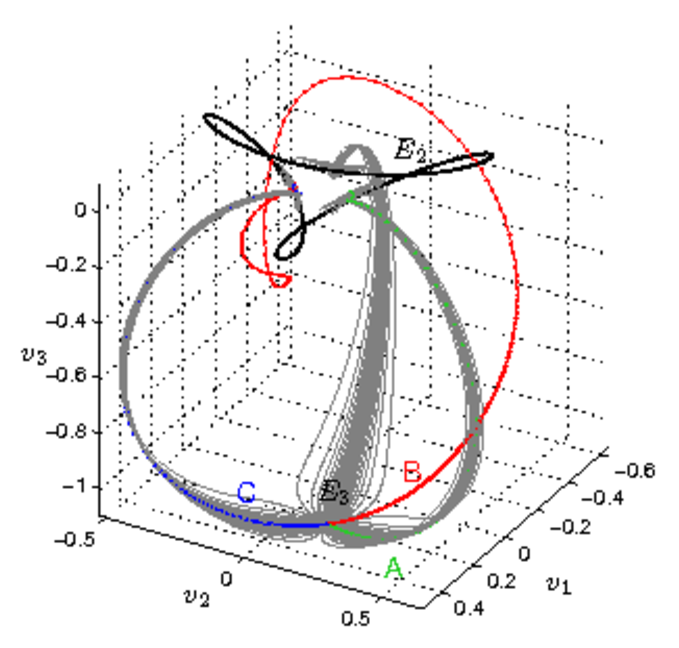
\includegraphics[width=0.45\textwidth, clip=true]{figs_bmp/ks22_E3_manifold.eps}
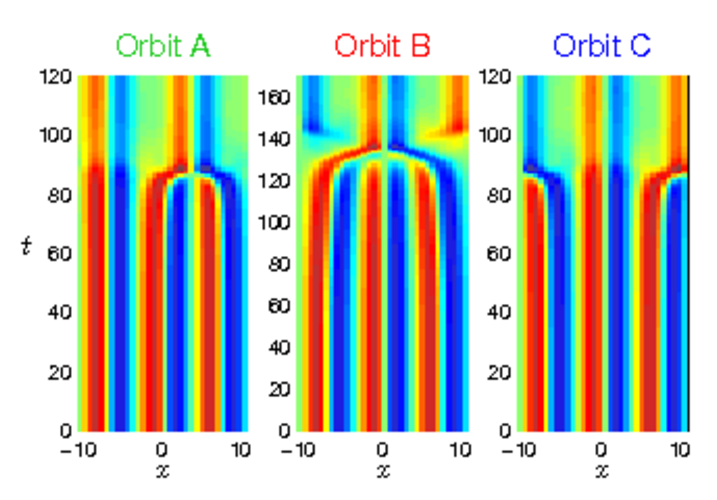
\includegraphics[width=0.5\textwidth, clip=true]{figs_bmp/ks22_E3_orbits_c.eps}
\end{center}
\caption{
The left panel shows the two-dimensional
unstable manifold of \eqv\ \EQV{3}. The coordinate axes
$v_1$, $v_2$, and $v_3$ are
projections onto three orthonormal vectors
$\mathbf{v}_1$, $\mathbf{v}_2$, and $\mathbf{v}_3$,
respectively, constructed from vectors
$\jEigvec{1}$, $\jEigvec{2}$, and $\jEigvec{4}$ by Gram-Schmidt orthogonalization.
The black line shows a family of \EQV{2}~\eqva\ related by translational
symmetry. The right panel shows spatial representation of
three orbits. Orbits $B$ and $C$ are two different heteroclinic orbits
connecting \EQV{3} to the same point on the \EQV{2} line.
        }
\label{f:KS22E3man}
\end{figure}
%%%%%%%%%%%%%%%%%%%%%%%%%%%%%%%%%%%%%%%%%%%%%%%%%%%%%%%%%%%%%%%%

Heteroclinic connections are non-generic for high-dimensional
systems, but can be robust in systems with continuous
symmetry, see \refref{KrupaRobHetCyc97} for a review.
Armbruster \etal\rf{AGHks89} study a fourth order truncation
of KS dynamics on the center-unstable manifold of $\EQV{2}$
close to a bifurcation off the constant $u(x,t)=0$ solution
and prove existence of a heteroclinic connection, see also
\refref{AGHO288}. Kevrekidis \etal\rf{KNSks90} study the
dynamics numerically and establish the existence of a robust
heteroclinic connection for a range of parameters close to
the onset of the 2-cell branch in terms of the symmetry and a
flow invariant subspace. We adopt their arguments to explain
the new heteroclinic connections
shown in \reffig{f:KS22hetero} that
we have found for $L=22$.
For our system size there are exactly two representatives of
the $\EQV{2}$ family that lie in the intersection of $\bbU^+$
and $\bbU^{(1)}$ related to each other by an $L/4$ shift.
Denote them by $\EQV{2}$ and $\Shift_{1/4}\EQV{2}$
respectively. The unstable eigenplane of $\EQV{2}$ lies on
$\bbU^+$ while that of $\Shift_{1/4}\EQV{2}$ lies on
$\bbU^{(1)}$, \cf\ \reftab{tab:Eksym}. The $\EQV{3}$ family
members that live in $\bbU^+$ have one of their unstable
eigenvectors (the one related to the heteroclinic connection
to $\EQV{2}$ family)  on $\bbU^+$, while the other does not
lie on symmetry-invariant subspace. Similarly, for the
$\EQV{1}$ family we observe that the equilibria in $\bbU^+$
have an unstable plane on $\bbU^+$ (again related to the
heteroclinic connection) and a second one with no symmetry.
Thus $\Shift_{1/4}\EQV{2}$ appears as a sink on $\bbU^+$,
while all other equilibria appear as sources. This explains
the heteroclinic connections from $\EQV{1}\,,\EQV{2}$ and
$\EQV{3}$ to $\Shift_{1/4}\EQV{2}$. Observing that
$\Shift_{1/4} \bbU^+= \bbU^{(1)}$ and taking into account
\reftab{tab:Eksym} we understand that within $\bbU^{(1)}$ we
have connections from $\Shift_{1/4}\EQV{2}$ (and members of
$\EQV{1}$ and $\EQV{3}$ families) to $\EQV{2}$ and the
formation of a heteroclinic loop. Due to the translational
invariance of KS there is a heteroclinic loop for any two
points of the $\EQV{2}$ family related by an $\Shift_{1/4}$-shift.

%%%%%%%%%%%%%%%%%%%%%%%%%%%%%%%%%%%%%%%%%%%%%%%%%%%%%%%%%%%%%%%%
\begin{figure}[t]
\begin{center}
        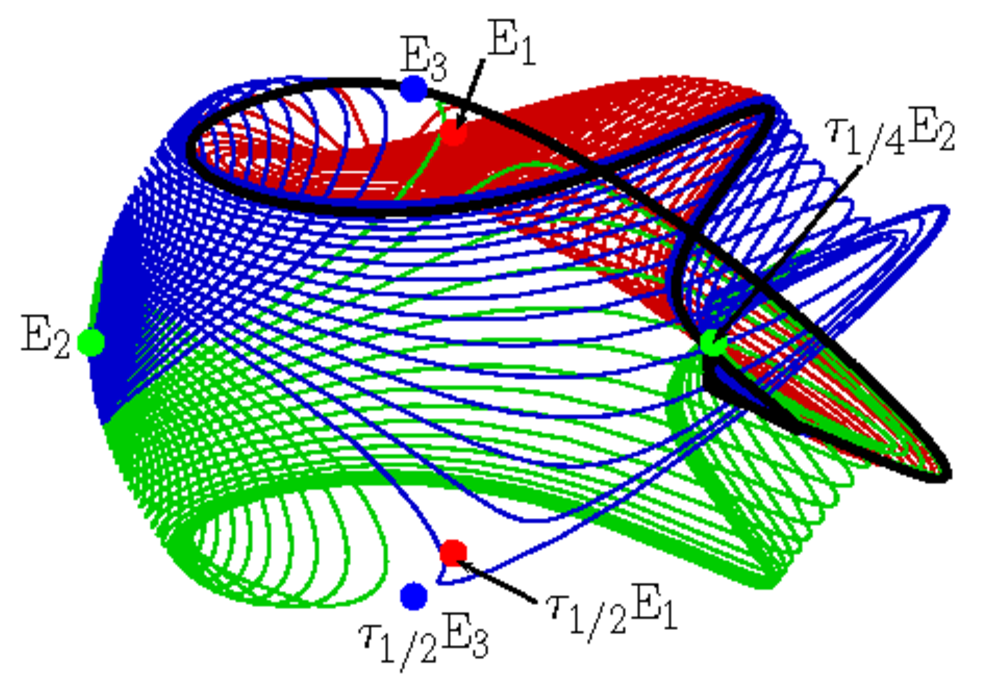
\includegraphics[width=0.6\textwidth, clip=true]{figs_bmp/KS22hetero.eps}
\end{center}
\caption{ Heteroclinic connections on $\bbU^+$:
 (red) The unstable manifold of \EQV{1}~\eqv.
 (blue/green) The unstable manifold of \EQV{2}~\eqv.
 (black) Heteroclinic connections from \EQV{3}~\eqv\ to $\Shift_{1/4}$\EQV{2}~\eqv,
 where $ \Shift_{1/m}u(x)=u(x+L/m)$ is a rational shift \refeq{eq:shiftFour}.
 Projection from $128$ dimensions onto the plane given by the vectors
 $a_{\EQV{2}}-a_{\Shift_{1/4}\EQV{2}}$ and $a_{\EQV{3}}-a_{\Shift_{1/2}\EQV{3}}$.}
\label{f:KS22hetero}
\end{figure}
%%%%%%%%%%%%%%%%%%%%%%%%%%%%%%%%%%%%%%%%%%%%%%%%%%%%%%%%%%%%%%%%%%



\section{\Rpo s for $L=22$}
\label{sec:rpos}

The \rpo s satisfy the condition \refeq{KSrpos}
$u(x+\shift_p,\period{p}) = u(x,0)$,
where $\period{p}$ is the period and $\shift_p$ the phase shift.
We have limited our search to orbits with $\period{p} < 200$ and found
over 30\,000 \rpo s with $\shift_p > 0$.  The details of the algorithm
used and the search strategy employed are given in
\refappe{sec:lmderRLD}.
Each \rpo\ with phase shift
$\shift_p > 0$ has a reflection symmetric partner
$u_p(x) \to -u_p(-x)$ with phase shift $-\shift_p$.

The small period \rpo s outline the coarse structure of the chaotic
attractor, while the longer period \rpo s resolve the finer details
of the dynamics.
The first four orbits with the shortest periods we have found are
shown in \reffig{f:ks22rpos}\,(\textit{a-d}).  The shortest \rpo\ with
$\period{p} = 16.4$ is also the most unstable, with one positive
Floquet exponent equal 0.328.  The other short orbits are less
unstable, with the largest Floquet exponent in the range
0.018 -- 0.073, typical of the long time attractor average.

%%%%%%%%%%%%%%%%%%%%%%%%%%%%%%%%%%%%%%%%%%%%%%%%%%%%%%%%%%%%%%%%
\begin{figure}[t]
\begin{center}
\begin{tabular}{cccccc} (\textit{a}) & (\textit{c}) & (\textit{e}) &
                        (\textit{g}) & (\textit{i}) & (\textit{k})\\
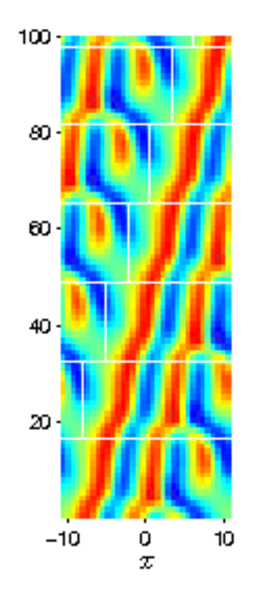
\includegraphics[width=0.15\textwidth, clip=true]{figs_bmp/ks22rpo016.3-02.86.eps}\hspace{-3ex} &
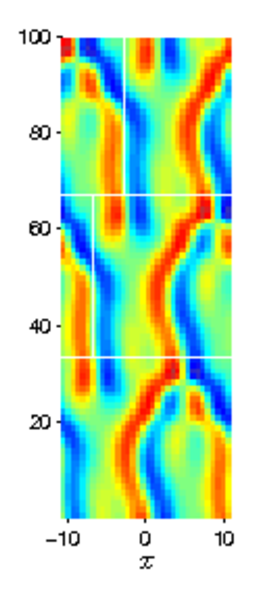
\includegraphics[width=0.15\textwidth, clip=true]{figs_bmp/ks22rpo033.5-04.04.eps}\hspace{-3ex} &
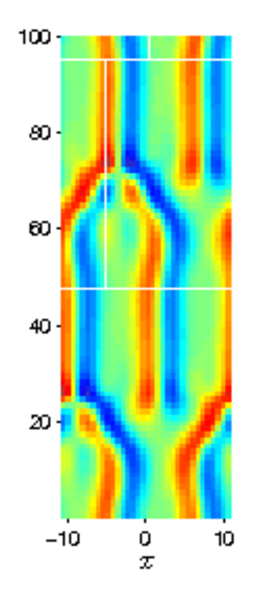
\includegraphics[width=0.15\textwidth, clip=true]{figs_bmp/ks22rpo047.6-05.68.eps}\hspace{-3ex} &
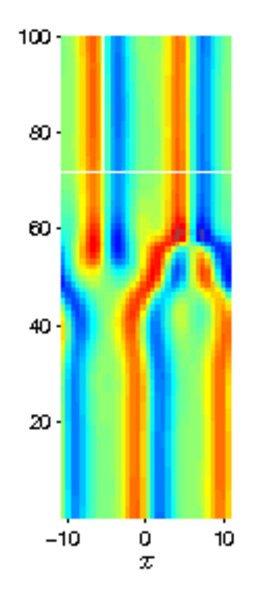
\includegraphics[width=0.15\textwidth, clip=true]{figs_bmp/ks22rpo071.7-05.50.eps}\hspace{-3ex} &
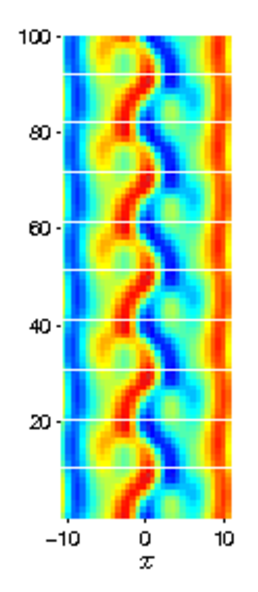
\includegraphics[width=0.15\textwidth, clip=true]{figs_bmp/ks22rpo020.5-00.00.eps}\hspace{-3ex} &
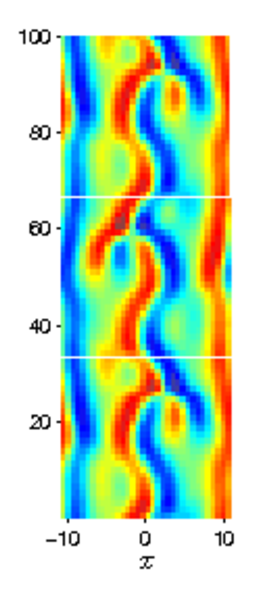
\includegraphics[width=0.15\textwidth, clip=true]{figs_bmp/ks22rpo066.8-00.00.eps}\\
(\textit{b}) & (\textit{d}) & (\textit{f}) &
(\textit{h}) & (\textit{j}) & (\textit{l})\\
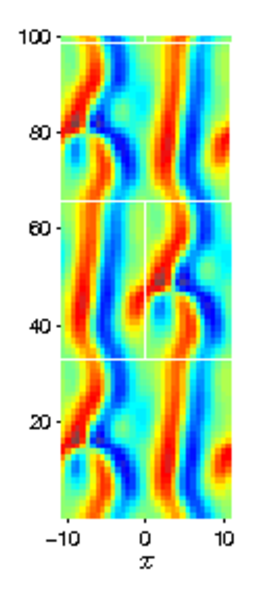
\includegraphics[width=0.15\textwidth, clip=true]{figs_bmp/ks22rpo032.8-10.96.eps}\hspace{-3ex} &
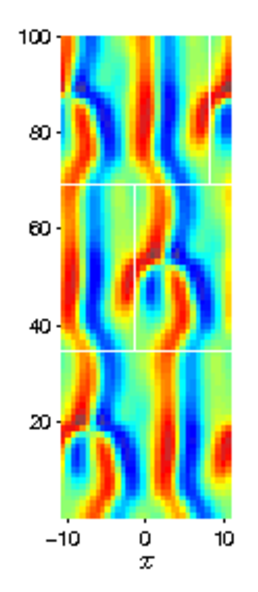
\includegraphics[width=0.15\textwidth, clip=true]{figs_bmp/ks22rpo034.6-09.60.eps}\hspace{-3ex} &
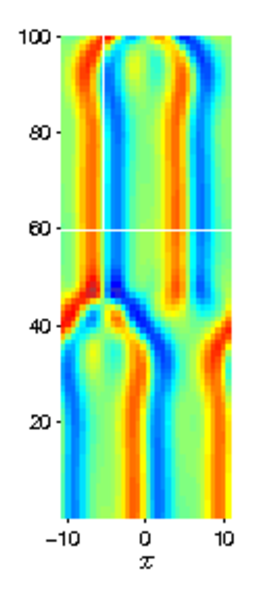
\includegraphics[width=0.15\textwidth, clip=true]{figs_bmp/ks22rpo059.9-05.44.eps}\hspace{-3ex} &
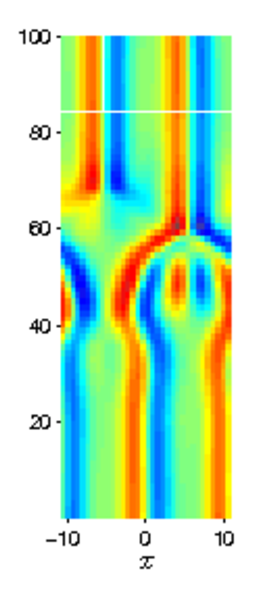
\includegraphics[width=0.15\textwidth, clip=true]{figs_bmp/ks22rpo084.4-05.51.eps}\hspace{-3ex} &
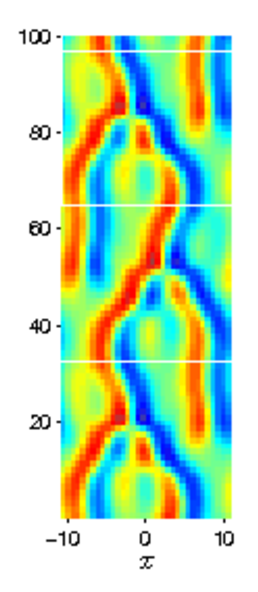
\includegraphics[width=0.15\textwidth, clip=true]{figs_bmp/ks22rpo064.7-00.00.eps}\hspace{-3ex} &
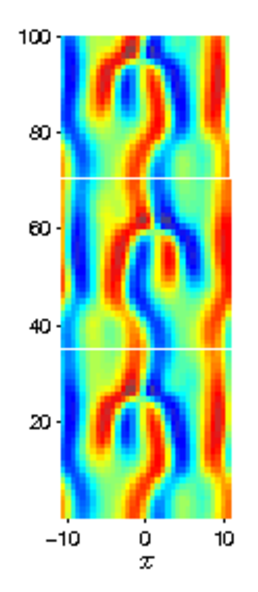
\includegraphics[width=0.15\textwidth, clip=true]{figs_bmp/ks22rpo070.3-00.00.eps}
\end{tabular}
\end{center}
\caption{Selected relative periodic and
pre-periodic
orbits of KS flow with $L = 22$:
(a) $\period{p} = 16.3$, $\shift_p = 2.86$;
(b) $\period{p} = 32.8$, $\shift_p = 10.96$;
(c) $\period{p} = 33.5$, $\shift_p = 4.04$;
(d) $\period{p} = 34.6$, $\shift_p = 9.60$;
(e) $\period{p} = 47.6$, $\shift_p = 5.68$;
(f) $\period{p} = 59.9$, $\shift_p = 5.44$;
(g) $\period{p} = 71.7$, $\shift_p = 5.503$;
(h) $\period{p} = 84.4$, $\shift_p = 5.513$;
(i) $\period{p} = 10.3$;
(j) $\period{p} = 32.4$;
(k) $\period{p} = 33.4$;
(l) $\period{p} = 35.2$.
Horizontal and vertical white lines indicate periodicity and phase
shift of the orbits, respectively.
}\label{f:ks22rpos}
\end{figure}
%%%%%%%%%%%%%%%%%%%%%%%%%%%%%%%%%%%%%%%%%%%%%%%%%%%%%%%%%%%%%%%%


We have found \rpo s which stay
close to the unstable manifold of \EQV{2}.
As is illustrated in \reffig{f:ks22rpos}\,(\textit{e-h}), all such orbits have
shift $\shift_p \approx L/4$, similar to the shift of orbits within
the unstable manifold of \EQV{2}, which start at \EQV{2} and
converge to $\Shift_{1/4}$\EQV{2} (see \reffig{f:KS22E2man}). This
confirms that the `cage' of unstable manifolds of equilibria plays
an important role in organizing the chaotic dynamics of the KS
equation.


\section{Pre-periodic orbits} \label{ssec:po}

As discussed in \refSect{sec:KSePO}, a \rpo\ will be
periodic, \ie, $\shift_p = 0$, if it either {\bf (a)} lives
within the $\bbU^+$ antisymmetric subspace, $-u(-x,0) =
u(x,0)$, or {\bf (b)} returns to its reflection
or its discrete rotation after a period:
$u(x,t+\period{p})=\gamma u(x,t)$, $\gamma^m=e$,
and is thus periodic with period $m\period{p}$.
The dynamics of KS flow in the antisymmetric subspace and \po
s with symmetry {\bf (a)} have been investigated
previously\rf{Christiansen97,LanThesis,lanCvit07}.
%     \PC{this seems to have vanished, but I remember citing the system
%     sizes: Vaggelis, if there is time please complete:
%     ``at system sizes $L=...$ and $L=...$.''}
The KS flow does not have any periodic orbits of this type
for $L = 22$.

Using the algorithm and strategy described in
\refappe{sec:lmderRLD}, we have found over 30\,000
pre-periodic orbits with $\period{p} < 200$ which possess the
symmetry of type {\bf (b)} with $\gamma=\Refl\in D_1$.
Some of the shortest such orbits we have found are shown in
\reffig{f:ks22rpos}\,(\textit{i-l}). Several were found as
repeats of pre-periodic orbits during searches for \rpo s
with non-zero shifts, while most have been found as solutions
of the pre-periodic orbit condition \refeq{KSpos} with
reflection, which takes form
\beq
 -\mathbf{g}(-\shift)a^\ast(\period{p}) = a(0)\,.
\label{KSposFour}
\eeq
in the Fourier space representation
(compare this to the condition \refeq{eq:system} for \rpo s).


\section{Energy transfer rates  for $L=22$}
\label{sec:energyL22}


%%%%%%%%%%%%%%%%%%%%%%%%%%%%%%%%%%%%%%%%%%%%%%%%%%%%%%%%%%%%%%%%
\begin{figure}[t]
\begin{center}
 \begin{tabular}{cc}
        ~~~~~~~~(\textit{a})                        &   ~~~~~~~~(\textit{b}) \\
    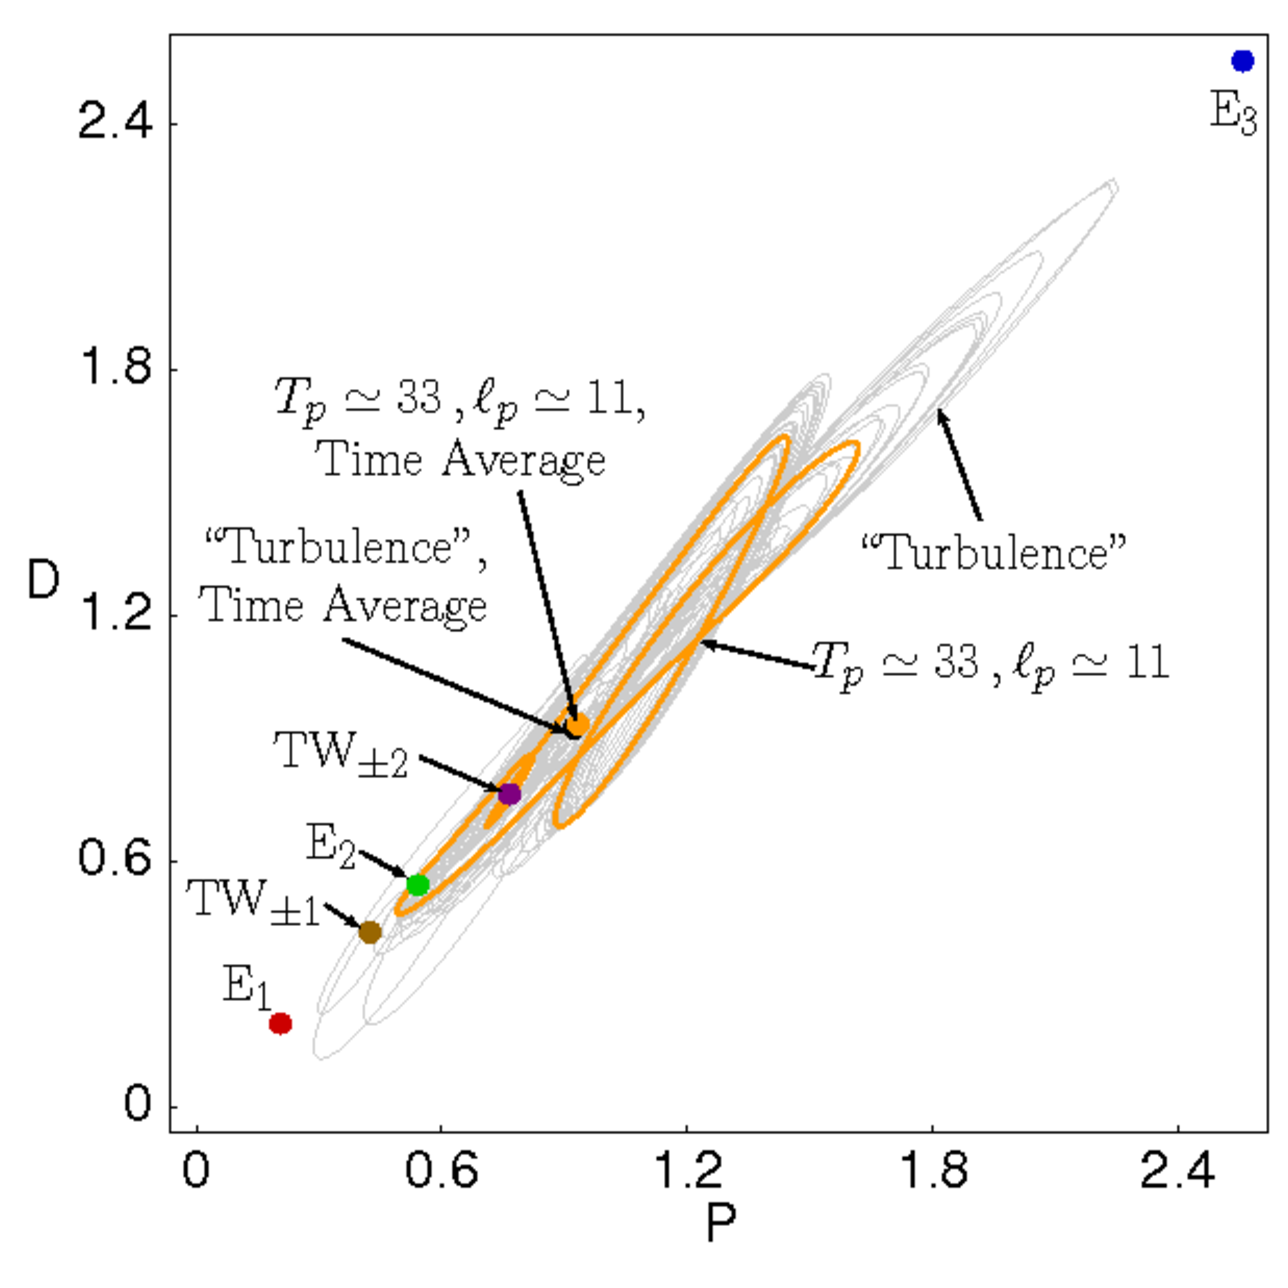
\includegraphics[width=0.46\textwidth, clip=true]{figs_bmp/energyBalance_pst.eps}  & 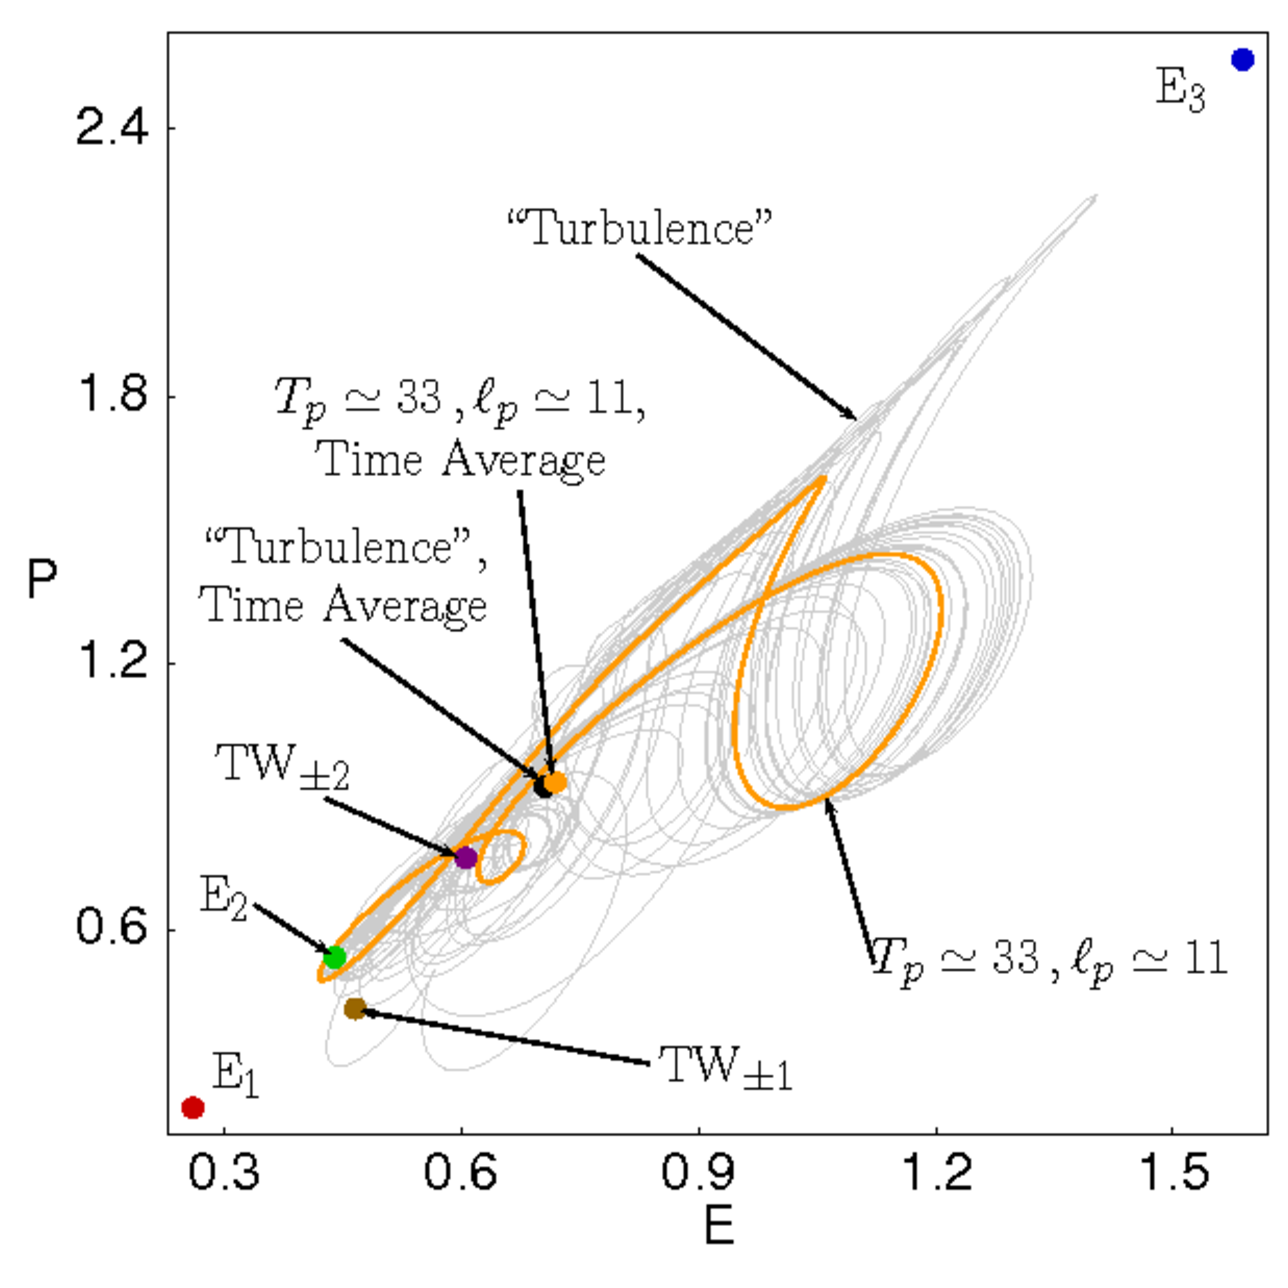
\includegraphics[width=0.46\textwidth, clip=true]{figs_bmp/equivaEP_pst.eps}

  \end{tabular}
\end{center}
\caption{
(a) Power input $P$ {\em vs.}
dissipation rate $D$
(b) energy $E$  {\em vs.}
power input $P$,   for several  \eqva\ and \reqva,
a \rpo, and a typical `turbulent' long-time trajectory.
Projections of the heteroclinic connections are
given in \reffig{f:drivedragConn}.
System size $L=22$.
        }
\label{f:drivedrag}
\end{figure}
%%%%%%%%%%%%%%%%%%%%%%%%%%%%%%%%%%%%%%%%%%%%%%%%%%%%%%%%%%%%%%%%%%

%%%%%%%%%%%%%%%%%%%%%%%%%%%%%%%%%%%%%%%%%%%%%%%%%%%%%%%%%%%%%%%%
\begin{figure}[t]
\begin{center}
 \begin{tabular}{cc}
        ~~~~~~~~(\textit{a})                        &   ~~~~~~~~(\textit{b}) \\
    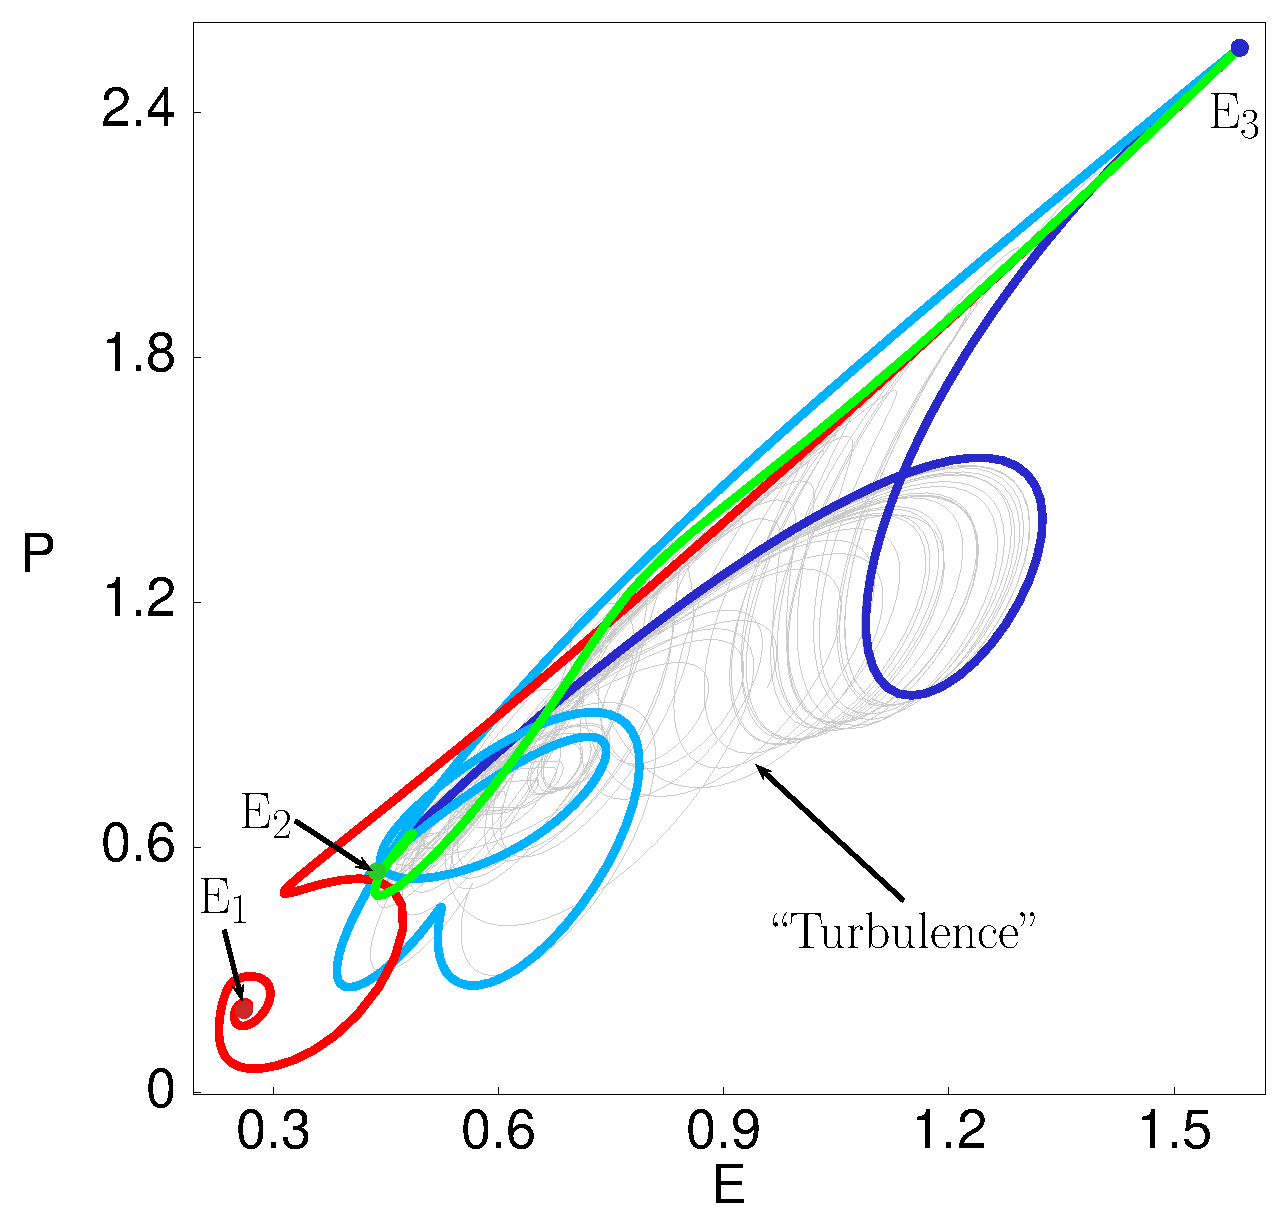
\includegraphics[width=0.46\textwidth, clip=true]{figs_bmp/connEP_pst.eps}     & 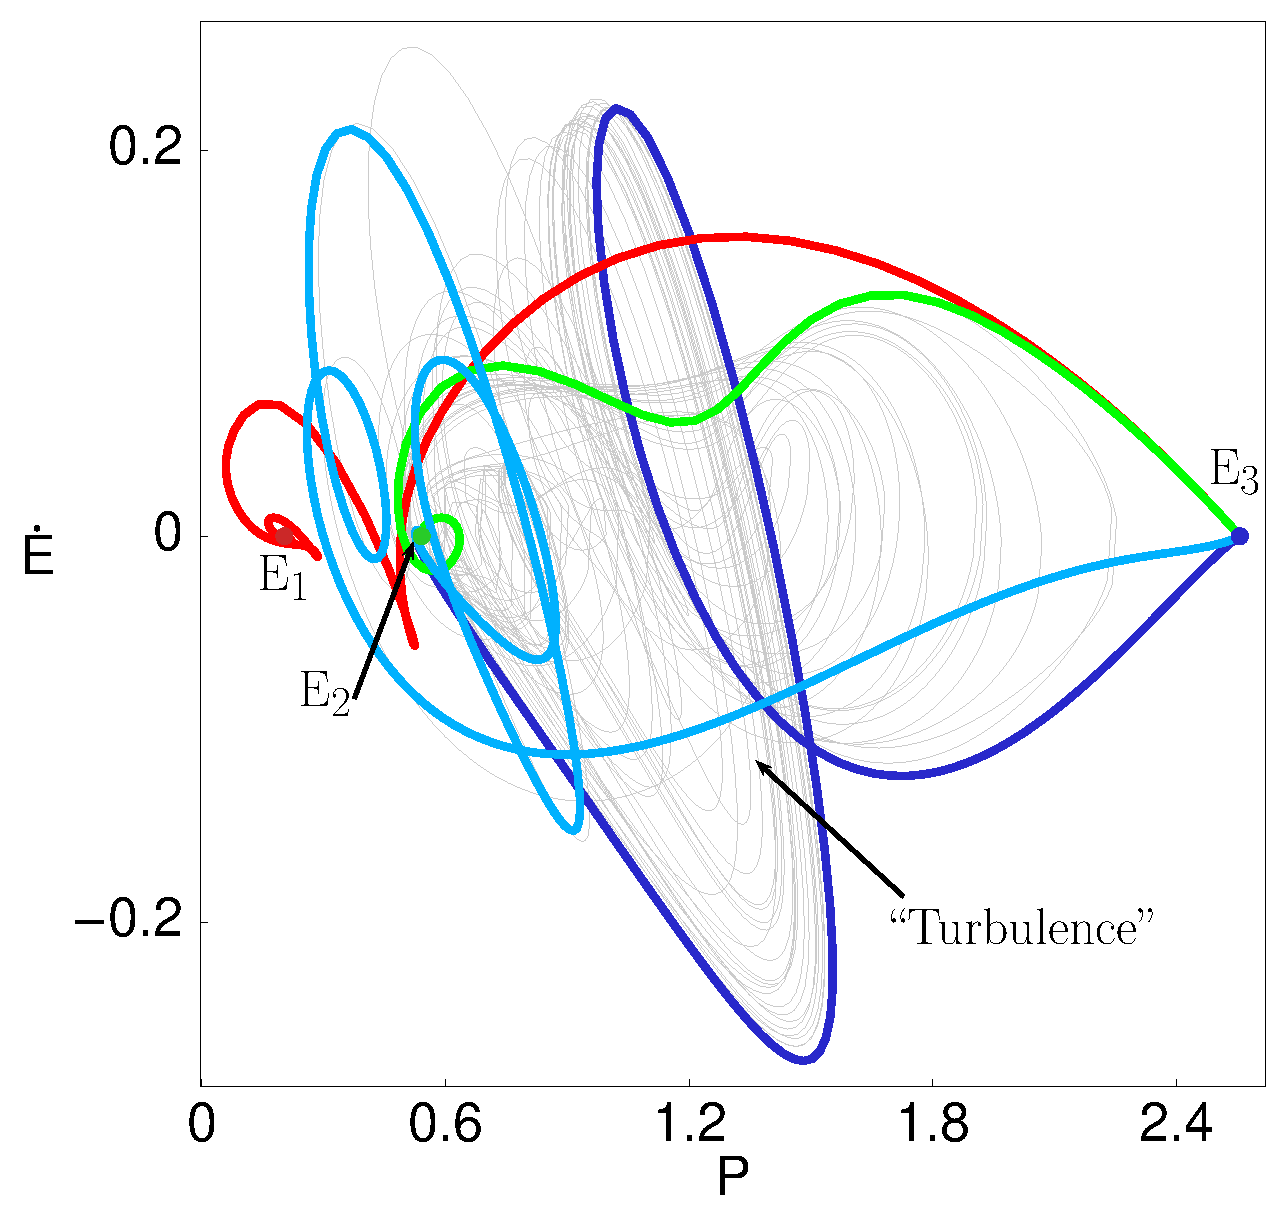
\includegraphics[width=0.46\textwidth, clip=true]{figs_bmp/connPEdot_pst.eps}
 \end{tabular}
\end{center}
\caption{
Two projections of the $(E,P,\dot{E})$ representation of the flow.
\EQV{1} (red), \EQV{2} (green), \EQV{3} (blue),
heteroclinic connections from \EQV{2} to $\EQV{3}$ (green),
from $\EQV{1}$ to \EQV{3} (red)
and from \EQV{3} to $\EQV{2}$ (shades of blue), superimposed over
a generic long-time `turbulent' trajectory (grey).
(a) As in \reffig{f:drivedragConn}\,(\textit{b}),
with labels omitted for clarity.
(b) A plot of  $\dot{\expctE} = P - D$ yields a clearer
visualization than \reffig{f:drivedragConn}\,(\textit{a}).
System size $L=22$.
        }
\label{f:drivedragConn}
\end{figure}
%%%%%%%%%%%%%%%%%%%%%%%%%%%%%%%%%%%%%%%%%%%%%%%%%%%%%%%%%%%%%%%%%%

In \reffig{f:drivedrag} we plot \refeq{EnRate}, the time-dependent
$\dot{\expctE}$ in the power input $P$ {\em vs.}
dissipation rate $D$ plane, for $L=22$ \eqva\ and \reqva,
a selected \rpo, and for a typical `turbulent' long-time
trajectory.

Projections from the $\infty$-dimensional \statesp\ onto the 3-dimensional
$(E,P,D)$ representation of the flow, such as
\reffigs{f:drivedrag}{f:drivedragConn}, can be misleading.
The most one can say is that if points are clearly separated in an
$(E,P,D)$ plot (for example, in \reffig{f:drivedrag}
$\EQV{1}$ \eqv\ is outside the recurrent set), they are also separated
in the full \statesp.  Converse is not true -- states of
very different topology can have similar energies.

An example is
the \rpo\ $(\period{p},\shift_p) = (32.8,10.96)$
(see \reffig{f:ks22rpos}\,(\textit{b})) which is the least
unstable short \rpo\ we have detected in this system. It appears to be
well embedded within the turbulent flow. The mean power $\timeAver{P_p}$ evaluated
as in \refeq{poE}, see \reffig{f:drivedrag},
is numerically quite close to the long-time
turbulent time average $\timeAver{P}$.
Similarly close prediction of mean dissipation rate in the
\pCf\ from a single-period \po\ computed by
Kawahara and Kida\rf{KawKida01} has lead to
optimistic hopes that `turbulence' is different from
low-dimensional chaos, insofar that the determination of one special
\po\ could yield all long-time averages.
Regrettably, not true -- as always, here too one needs a hierarchy
of \po s of increasing length to obtain accurate
predictions\rf{DasBuch}.

%%%%%%%%%%%%%%%%%%%%%%%%%%%%%%%%%%%%%%%%%%%%%%%%%%%%%%%%%%%%%%%%
\begin{figure}[t]
\begin{center}
(\textit{a})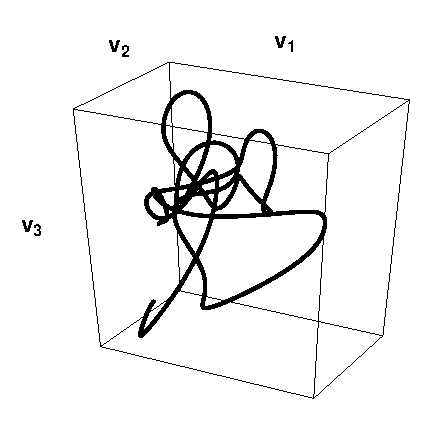
\includegraphics[width=0.46\textwidth, clip=true]{figs_bmp/ks22rpo033.50_04.045E2.eps}
(\textit{b})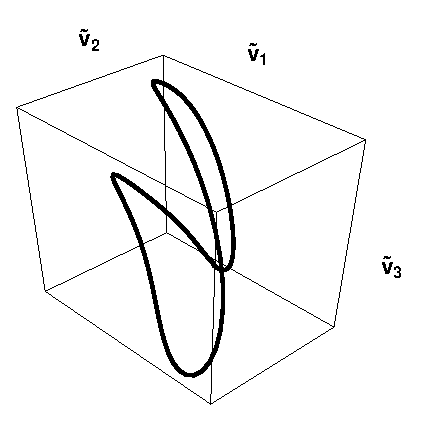
\includegraphics[width=0.46\textwidth, clip=true]{figs_bmp/ks22rpo033.50_04.045E2CM.eps}
\\
\end{center}
\caption{
 The
\rpo\ with $(\period{p},\shift_p) =(33.5,4.04)$
from \reffig{f:ks22rpos}\,(\textit{c})
which appears well embedded within the turbulent flow:
 (a) A stationary \statesp\ projection,
  traced for four periods $\period{p}$. The coordinate axes
$v_1$, $v_2$, and $v_3$ are those of \reffig{f:KS22E2man};
 (b) In the co-moving mean velocity frame.
%PC dropped this: traced for one period $\period{p}$.
        } \label{f:MeanVelocityFrame}
\end{figure}
%%%%%%%%%%%%%%%%%%%%%%%%%%%%%%%%%%%%%%%%%%%%%%%%%%%%%%%%%%%%%%%%%%

For any given \rpo\ a convenient visualization is
offered by the {\em mean velocity frame}, {\ie},
a reference frame that rotates with velocity
$\velRel_p=\shift_p/\period{p}$.
In the mean velocity frame a \rpo\ becomes
a \po, as in \reffig{f:MeanVelocityFrame}\,(\textit{b}).
However, each {\rpo} has its own mean velocity frame and thus
sets of \rpo s are difficult to visualize simultaneously.
